\appendix
\addcontentsline{toc}{chapter}{Appendices}

\singlespacing

\chapter{Materials and Methods}\label{app:Methods}
\begin{center}
\begin{landscape}

\begin{table}[htbp]
\begin{tabular}{|l|l|l|l|}
\hline
Organism               & Amplicon & Primer/probe                                                                           & Nucleotide sequence                                                                                                                                                               \\ \hline
\textit{S. pneumoniae} & 67 bp         & \begin{tabular}[c]{@{}l@{}}Taqman probe\\ Forward primer\\ Reverse primer\end{tabular} & \begin{tabular}[c]{@{}l@{}}5'-/5HEX/AAT GTT ACG/ZEN/CAA CTG ACG AG/3IABkFQ/-3'\\ 5'-GCT GTT TTA GCA GAT AGT GAG ATC GA-3'\\ 5'-TCC CAG TCG GTG CTG TCA-3'\end{tabular}            \\ \hline
Influenza A            & 185 bp        & \begin{tabular}[c]{@{}l@{}}Taqman probe\\ Forward primer\\ Reverse primer\end{tabular} & \begin{tabular}[c]{@{}l@{}}5'-/56-FAM/TGC AGT CCT/ZEN/CGC TCA CTG GGC ACG /3IABkFQ/-3'\\ 5'-AGG GCA TTY TGG ACA AAK CGT CTA-3'\\ 5'-GAC CRA TCC TGT CAC CTC TGA C-3'\end{tabular} \\ \hline
Epstein-Barr virus     & 75 bp         & \begin{tabular}[c]{@{}l@{}}Taqman probe\\ Forward primer\\ Reverse primer\end{tabular} & \begin{tabular}[c]{@{}l@{}}5'-/56-FAM/AGG GAG ACA/ZEN/CAT CTG GAC CAG AAG GC/3IABkFQ/-3'\\ 5'-TCT TTG AGG TCC ACT GCC G-3'\\ 5'-TAC AGG ACC TGG AAA TGG CC-3'\end{tabular}       \\ \hline
Cytomegalovirus        & 66 bp         & \begin{tabular}[c]{@{}l@{}}Taqman probe\\ Forward primer\\ Reverse primer\end{tabular} & \begin{tabular}[c]{@{}l@{}}5'-/56-FAM/TG GGC AAC C/ZEN/A CCG CAC TGA GG/3IABkFQ/-3'\\ 5'-TGG GCG AGG ACA ACG AA-3'\\ 5'-TGA GGC TGG GAA GCT GAC AT-3'\end{tabular}                \\ \hline
\end{tabular}
\medskip
\caption[Primer/probe sets used for the digital droplet PCR experiments]{\textbf{Primer/probe sets used for the digital droplet PCR experiments}}
\label{tab:ddPCRprobes}
\end{table}
\end{landscape}
\bigskip
\newpage





\chapter{Application of Metagenomic Sequencing to Sepsis Samples}
\label{app:Results1}


\begin{table}[]
\scalebox{0.7}{
\begin{tabular}{|l|l|}
\hline
\textbf{Virus family} & \textbf{Virus species}                                                                                                                                                                                                                                                                                   \\ \hline
Adenoviridae          & Human adenovirus                                                                                                                                                                                                                                                                                         \\ \hline
Arenaviridae          & \begin{tabular}[c]{@{}l@{}}Lassa virus\\ Lymphocytic choriomeningitis virus\end{tabular}                                                                                                                                                                                                                 \\ \hline
Coronaviridae         & \begin{tabular}[c]{@{}l@{}}Human coronavirus HKU1, NL63, OC43, 229E\\ Middle East respiratory syndrome coronavirus\\ Severe acute respiratory syndrome coronavirus\end{tabular}                                                                                                                          \\ \hline
Flaviviridae          & \begin{tabular}[c]{@{}l@{}}Dengue virus\\ Japanese encephalitis virus\\ Murray Valley encephalitis virus\\ St Louis encephalitis virus\\ Tick-borne encephalitis virus\\ West Nile virus\\ Yellow fever virus\\ Zika virus\end{tabular}                                                                  \\ \hline
Herpesviridae         & \begin{tabular}[c]{@{}l@{}}Human herpesvirus 3 (Varicella zoster virus)\\ Human herpesvirus 4 (Epstein Barrvirus)\\ Human herpesvirus 5 (Cytomegalovirus)\\ Human herpesvirus 6-7 (Roseolovirus)\\ Human herpesvirus 8 (Kaposi's sarcoma-associated herpesvirus)\\ Herpes simplex virus 1-2\end{tabular} \\ \hline
Orthomyxoviridae      & Influenza virus A-C                                                                                                                                                                                                                                                                                      \\ \hline
Paramyxoviridae       & \begin{tabular}[c]{@{}l@{}}Hendra henipavirus\\ Human metapneumovirus \\ Humanparainfluenzavirus1-5\\ Measles morbilivirus\\ Mumps rubulavirus\\ Nipah henipavirus\\ Respiratory syncytial virus \\ Sosugavirus\end{tabular}                                                                             \\ \hline
Parvoviridae          & \begin{tabular}[c]{@{}l@{}}Human bocavirus\\ Human parvovirus B19\\ Human parvovirus 4\\ Primate erythroparvovirus 1\\ Primate tetraparvovirus 1\end{tabular}                                                                                                                                            \\ \hline
Peribunyaviridae      & California encephalitis virus                                                                                                                                                                                                                                                                            \\ \hline
Phenuiviridae         & \begin{tabular}[c]{@{}l@{}}Rift valley fever virus\\ Sandfly fever Naples virus\\ Sandfly fever Sicilian virus\end{tabular}                                                                                                                                                                              \\ \hline
Picornaviridae        & \begin{tabular}[c]{@{}l@{}}Cardiovirus A-B\\ Coxsackie A virus\\ ECHO virus\\ Enterovirus A, B, D\\ Hepatitis A virus\\ Parechovirus A-B \\ Rhinovirus A-C\\ Rosavirus A\\ Salivivirus\end{tabular}                                                                                                      \\ \hline
Polyomaviridae        & \begin{tabular}[c]{@{}l@{}}BK virus\\ JC polyomavirus\end{tabular}                                                                                                                                                                                                                                       \\ \hline
Reoviridae            & Rotavirus A-C                                                                                                                                                                                                                                                                                            \\ \hline
Rhabdovirus           & \begin{tabular}[c]{@{}l@{}}Australian bat lyssavirus\\ Duvenhage lyssavirus\\ European bat lyssavirus 1-2\\ Lagos bat lyssavirus\\ Mokola lyssavirus\\ Rabies lyssavirus\end{tabular}                                                                                                                    \\ \hline
Togaviridae           & \begin{tabular}[c]{@{}l@{}}Chikungunya virus\\ Eastern equine encephalitis virus\\ Rubella virus\\ Venezuelan equine encephalitis virus\\ Western equine encephalitis virus\end{tabular}                                                                                                                 \\ \hline
\end{tabular}
}
\caption[Enrichment Probe Set Viruses]{\textbf{Viruses included in enrichment probe set}}
\label{tab:ProbeSetViruses}
\end{table}

\begin{table}[]
\begin{tabular}{|l|l|}
\hline
\textbf{Bacterial genus}  & \textbf{Bacterial species}                                                             \\ \hline
\textit{Acinetobacter}    & \textit{\begin{tabular}[c]{@{}l@{}}baumanii\\ calcoaceticus\end{tabular}}              \\ \hline
\textit{Bartonella}       & \textit{henselae}                                                                      \\ \hline
\textit{Bordetella}       & \textit{pertussis}                                                                     \\ \hline
\textit{Borrelia}         & \textit{burgdorferi}                                                                   \\ \hline
\textit{Brucella}         & \textit{}                                                                              \\ \hline
\textit{Burkholderia}     & \textit{cepacia}                                                                       \\ \hline
\textit{Chlamydophila}    & \textit{\begin{tabular}[c]{@{}l@{}}pneumoniae\\ psittaci\end{tabular}}                 \\ \hline
\textit{Coxiella}         & \textit{burnetii}                                                                      \\ \hline
\textit{Enterobacter}     & \textit{\begin{tabular}[c]{@{}l@{}}aerogenes\\ cloacae\end{tabular}}                   \\ \hline
\textit{Escherichia}      & \textit{coli}                                                                          \\ \hline
\textit{Haemophilus}      & \textit{\begin{tabular}[c]{@{}l@{}}influenzae\\ parainfluenzae\end{tabular}}           \\ \hline
\textit{Klebsiella}       & \textit{\begin{tabular}[c]{@{}l@{}}pneumoniae\\ oxytoca\end{tabular}}                  \\ \hline
\textit{Legionella}       & \textit{pneumophila}                                                                   \\ \hline
\textit{Leptospira}       & \textit{}                                                                              \\ \hline
\textit{Listeria}         & \textit{monocytogenes}                                                                 \\ \hline
\textit{Moraxella}        & \textit{catarrhalis}                                                                   \\ \hline
\textit{Mycobacterium}    & \textit{\begin{tabular}[c]{@{}l@{}}avium\\ intracellulare\\ tuberculosis\end{tabular}} \\ \hline
\textit{Mycoplasma}       & \textit{pneumoniae}                                                                    \\ \hline
\textit{Neisseria}        & \textit{meningitidis}                                                                  \\ \hline
\textit{Nocardia}         & \textit{}                                                                              \\ \hline
\textit{Pseudomonas}      & \textit{aeruginosa}                                                                    \\ \hline
\textit{Serratia}         & \textit{marcescens}                                                                    \\ \hline
\textit{Staphylococcus}   & \textit{aureus}                                                                        \\ \hline
\textit{Stenotrophomonas} & \textit{maltophilia}                                                                   \\ \hline
\textit{Streptococcus}    & \textit{\begin{tabular}[c]{@{}l@{}}agalactiae\\ pneumoniae\\ pyogenes\end{tabular}}    \\ \hline
\textit{Treponema}        & \textit{pallidum}                                                                      \\ \hline
\end{tabular}
\caption[Enrichment Probe Set Bacteria]{\textbf{Bacteria included in enrichment probe set}}
\label{tab:ProbeSetBacteria}
\end{table}




\begin{landscape}


\begin{table}[]
\centering
\caption[Viral Multiplex Reference]{Viral Multiplex Reference reagent 11/242 (UK NIBSC). This reference set included 25 viruses of various nucleic acid types, envelope types and genome sizes. 21/25 viruses had corresponding enrichment probes in our probe panel. (Adapted from Mee et al.)
\label{tab:VMR}\\
{\bf }}
\scalebox{0.85}{
\begin{tabular}{|l|l|l|l|l|l|l|}
\hline
Group                      & Family                            & Species/serotype               & Envelope             & Genome size & Included in probeset & Concentration (log10 copies/ml) \\ \hline
\multirow{7}{*}{dsDNA}     & \multirow{2}{*}{Adenoviridae}     & Adenovirus 2                   & \multirow{2}{*}{No}  & 35.9        & Yes                  & NA                                           \\ \cline{3-3} \cline{5-7} 
                           &                                   & Adenovirus 41                  &                      & 34.2        & Yes                  & NA                                           \\ \cline{2-7} 
                           & \multirow{5}{*}{Herpesviridae}    & Human herpesvirus 1            & \multirow{5}{*}{Yes} & 151.2       & Yes                  & NA                                           \\ \cline{3-3} \cline{5-7} 
                           &                                   & Human herpesvirus 2            &                      & 154.7       & Yes                  & NA                                           \\ \cline{3-3} \cline{5-7} 
                           &                                   & Human herpesvirus 3 (VZV)      &                      & 124.8       & Yes                  & NA                                           \\ \cline{3-3} \cline{5-7} 
                           &                                   & Human herpesvirus 4 (EBV)      &                      & 171.7       & Yes                  & 3.88                                         \\ \cline{3-3} \cline{5-7} 
                           &                                   & Human herpesvirus 5 (CMV)      &                      & 233.7       & Yes                  & 4.66                                         \\ \hline
dsRNA                      & Reoviridae                        & Rotavirus A                    & No                   & 18.5        & Yes                  & 6.76                                         \\ \hline
\multirow{8}{*}{ssRNA (+)} & Astroviridae                      & Astrovirus                     & No                   & 6.8         & No                   & NA                                           \\ \cline{2-7} 
                           & \multirow{3}{*}{Caliciviridae}    & Norovirus GI                   & \multirow{3}{*}{No}  & 7.6         & No                   & NA                                           \\ \cline{3-3} \cline{5-7} 
                           &                                   & Norovirus GII                  &                      & 7.5         & No                   & NA                                           \\ \cline{3-3} \cline{5-7} 
                           &                                   & Sapovirus C12                  &                      & 7.5         & No                   & NA                                           \\ \cline{2-7} 
                           & Coronaviridae                     & Coronavirus 229E               & Yes                  & 27.2        & Yes                  & NA                                           \\ \cline{2-7} 
                           & \multirow{3}{*}{Picornaviridae}   & Coxsackievirus B4              & \multirow{3}{*}{No}  & 7.4         & Yes                  & NA                                           \\ \cline{3-3} \cline{5-7} 
                           &                                   & Rhinovirus A39                 &                      & 7.1         & Yes                  & NA                                           \\ \cline{3-3} \cline{5-7} 
                           &                                   & Parechovirus 3                 &                      & 7.2         & Yes                  & 7.07                                         \\ \hline
\multirow{9}{*}{ssRNA (-)} & \multirow{3}{*}{Orthomyxoviridae} & Influenza A virus H1N1         & \multirow{3}{*}{Yes} & 13.2        & Yes                  & NA                                           \\ \cline{3-3} \cline{5-7} 
                           &                                   & Influenza A virus H3N2         &                      & 13.6        & Yes                  & NA                                           \\ \cline{3-3} \cline{5-7} 
                           &                                   & Influenza B virus              &                      & 14.2        & Yes                  & NA                                           \\ \cline{2-7} 
                           & \multirow{6}{*}{Paramyxoviridae}  & Metapneumovirus A              & \multirow{6}{*}{Yes} & 13.3        & Yes                  & NA                                           \\ \cline{3-3} \cline{5-7} 
                           &                                   & Parainfluenzavirus 1           &                      & 15.5        & Yes                  & NA                                           \\ \cline{3-3} \cline{5-7} 
                           &                                   & Parainfluenzavirus 2           &                      & 15.7        & Yes                  & NA                                           \\ \cline{3-3} \cline{5-7} 
                           &                                   & Parainfluenzavirus 3           &                      & 15.4        & Yes                  & NA                                           \\ \cline{3-3} \cline{5-7} 
                           &                                   & Parainfluenzavirus 4           &                      & 17.4        & Yes                  & NA                                           \\ \cline{3-3} \cline{5-7} 
                           &                                   & Respiratory syncytial virus A2 &                      & 15.2        & Yes                  & 3.75                                         \\ \hline
\small
\end{tabular}
}
\end{table}


\end{landscape}

\clearpage

\end{center}

\chapter{Improved Classification of Microbiological Aetiology in Sepsis}
\label{ch:AppResults2}
\begin{figure}[htbp]
\centering
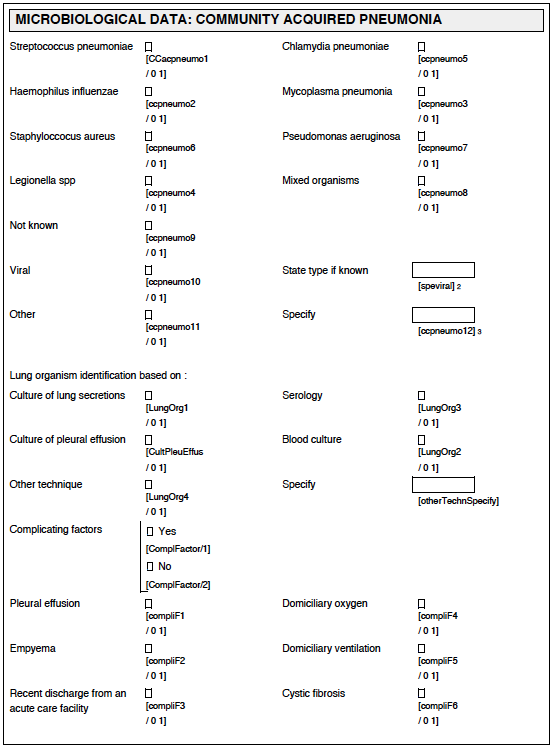
\includegraphics[scale=0.7]{./Appendices/Images/eCRF1.png}
\end{figure}

\begin{figure}[htbp]
\centering
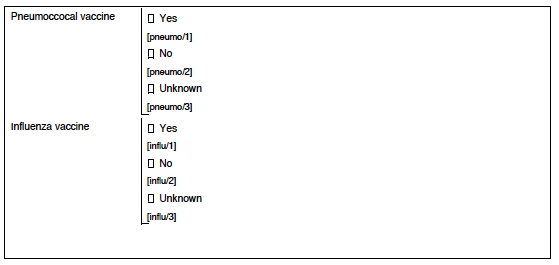
\includegraphics[scale=0.7]{./Appendices/Images/eCRF2.png}
\caption[Electronic case record form]{\textbf{GAinS electronic case record form: microbiology section}}
\label{fig:eCRF}
\end{figure}

\chapter{Integration of Microbiology with the Host Response}\label{ch:AppResults3}

\begin{table}[]
\begin{center}
\begin{tabular}{lll}
\textbf{Gene}      & \textbf{log2(fold change)} & \textbf{FDR} \\
\textit{IGLL1}     & 0.79                       & 4.02E-03     \\
\textit{CDC20}     & 0.62                       & 4.51E-03     \\
\textit{CACNA2D3}  & -0.63                      & 5.21E-03     \\
\textit{TXNDC5}    & 0.75                       & 8.48E-03     \\
\textit{IGKV3D-20} & 0.78                       & 9.23E-03     \\
\textit{KIAA0101}  & 0.59                       & 1.28E-02     \\
\textit{IGKV1D-33} & 0.61                       & 1.33E-02     \\
\textit{IGJ}       & 0.83                       & 1.33E-02     \\
\textit{PRTN3}     & 0.66                       & 4.68E-02    
\end{tabular}
\end{center}
\caption[Differentially expressed genes in EBV reactivation]{\textbf{Summary of differentially expressed genes in EBV-positive vs EBV-negative individuals.} Nine genes were significant at fold-change $>$1.5 and FDR $<$0.05.} 
\label{tab:ebv-de-genes}
\end{table}

\begin{table}[]
\begin{center}
\begin{tabular}{lll}
\textbf{Gene}      & \textbf{log2(fold change)} & \textbf{FDR} \\
\textit{IGLL1}     & 0.85                       & 1.15E-03     \\
\textit{TXNDC5}    & 0.81                       & 2.43E-03     \\
\textit{IGKV3D-20} & 0.84                       & 2.54E-03     \\
\textit{IGKV1D-33} & 0.66                       & 3.38E-03     \\
\textit{CDC20}     & 0.59                       & 3.98E-03     \\
\textit{IGJ}       & 0.89                       & 4.06E-03     \\
\textit{MGC29506}  & 0.61                       & 5.96E-03     \\
\textit{TNFRSF17}  & 0.63                       & 1.32E-02     \\
\textit{DEFA1B} & 0.82                       & 3.11E-02     \\
\textit{PRTN3}     & 0.66                       & 3.87E-02     \\
\textit{DEFA4}     & 0.75                       & 4.19E-02     \\
\textit{CEACAM6}   & 0.63                       & 4.82E-02    
\end{tabular}
\end{center}
\caption[Differentially expressed genes in EBV reactivation with SRS as a covariate]{\textbf{Summary of differentially expressed genes in EBV-positive vs EBV-negative individuals with SRS included as a covariate in the linear model.} Twelve genes were significant at fold-change $>$1.5 and FDR $<$0.05.} 
\label{tab:ebv-de-genes-srs}
\end{table}



\begin{table}
\begin{center}
\scalebox{0.9}{
\begin{tabular}{lll}
\textbf{Gene}      & \textbf{log2(fold change)} & \textbf{FDR} \\
\textit{IFI27}     & 3.10           & 6.88E-07           \\
\textit{IMPA2}     & -0.64          & 1.86E-04           \\
\textit{C3ORF54}   & 0.74           & 6.59E-04           \\
\textit{SPATS2L}   & 1.02           & 6.59E-04           \\
\textit{LOC554203} & 0.59           & 6.91E-04           \\
\textit{HERC6}     & 0.94           & 8.17E-04           \\
\textit{JUP}       & 1.28           & 9.63E-04           \\
\textit{TIMM10}    & 1.33           & 1.03E-03           \\
\textit{SRC}       & 0.77           & 1.03E-03           \\
\textit{HES4}      & 1.04           & 1.03E-03           \\
\textit{LGALS3BP}  & 0.82           & 1.03E-03           \\
\textit{RASGRP3}   & 0.75           & 1.03E-03           \\
\textit{TGIF2}     & 0.64           & 1.03E-03           \\
\textit{MT1A}      & 0.89           & 1.03E-03           \\
\textit{C9ORF91}   & 0.75           & 1.03E-03           \\
\textit{OAS1}      & 1.42           & 1.08E-03           \\
\textit{SCO2}      & 0.92           & 1.08E-03           \\
\textit{HS.125087} & 1.21           & 1.08E-03           \\
\textit{PARP12}    & 1.07           & 1.08E-03           \\
\textit{EPSTI1}    & 2.02           & 1.08E-03           \\
\textit{OAS2}      & 1.57           & 1.08E-03           \\
\textit{IFI44L}    & 2.42           & 1.08E-03           \\
\textit{SP140}     & 0.78           & 1.08E-03           \\
\textit{LY6E}      & 1.69           & 1.11E-03           \\
\textit{CXCL10}    & 0.78           & 1.16E-03           \\
\textit{TMCO3}     & -0.70          & 1.21E-03           \\
\textit{HS.72010}  & 0.63           & 1.28E-03           \\
\textit{XAF1}      & 1.44           & 1.28E-03           \\
\textit{IFI44}     & 1.68           & 1.33E-03           \\
\textit{RNASE1}    & 0.94           & 1.36E-03           \\
\textit{GALM}      & 0.85           & 1.45E-03           \\
\textit{IFIT3}     & 1.57           & 1.45E-03           \\
\textit{RSAD2}     & 1.81           & 1.84E-03           \\
\textit{LAMP3}     & 0.72           & 1.99E-03           \\
\textit{HS.386275} & 0.70           & 1.99E-03           \\
\textit{PLB1}      & -0.74          & 2.02E-03           \\
\textit{MT2A}      & 1.00           & 2.14E-03           \\
\textit{SERPING1}  & 1.50           & 2.14E-03           \\
\textit{OAS3}      & 1.66           & 2.14E-03           \\
\textit{CDKN1A}    & 0.71           & 2.14E-03           \\
\textit{LHFPL2}    & 0.68           & 2.30E-03           \\
\textit{BTN3A3}    & 0.85           & 2.47E-03           \\
\textit{PARP14}    & 0.95           & 2.52E-03           \\
\textit{IFIT5}     & 0.97           & 2.57E-03           \\
\textit{FHL2}      & 0.61           & 2.60E-03           \\
\textit{CXCL16}    & -0.63          & 2.93E-03           \\
\textit{SIGLEC10}  & -0.88          & 3.13E-03           \\
\textit{NLRC4}     & -0.67          & 3.55E-03           \\
\textit{ISG15}     & 1.68           & 3.59E-03           \\
\textit{ZNF684}    & 0.60           & 3.63E-03                  


\end{tabular}}
\end{center}
\caption[Differentially expressed genes in viral infection]{\textbf{Summary of differentially expressed genes in viral vs bacterial infection.} The top 50 most significantly differentially expressed genes are listed here.} 
\label{tab:vb-de-genes}
\end{table}

\begin{table}[]
\begin{center}
\scalebox{0.9}{
\begin{tabular}{lll}
\textbf{Gene}      & \textbf{log2(fold change)} & \textbf{FDR} \\
\textit{IFI27}     & 3.52                       & 1.3E-06      \\
\textit{JUP}       & 1.68                       & 2.0E-04      \\
\textit{C3ORF54}   & 0.90                       & 4.7E-04      \\
\textit{NPL}       & -0.66                      & 7.9E-04      \\
\textit{SPATS2L}   & 1.17                       & 1.1E-03      \\
\textit{CBL}       & -0.68                      & 1.4E-03      \\
\textit{IMPA2}     & -0.67                      & 1.7E-03      \\
\textit{HERC6}     & 1.01                       & 4.8E-03      \\
\textit{LGALS3BP}  & 0.89                       & 5.1E-03      \\
\textit{HES4}      & 1.12                       & 6.0E-03      \\
\textit{MT1A}      & 0.98                       & 6.2E-03      \\
\textit{BCAT1}     & -1.20                      & 7.0E-03      \\
\textit{RASGRP3}   & 0.80                       & 7.0E-03      \\
\textit{ECHDC3}    & -1.25                      & 7.2E-03      \\
\textit{CDC123}    & -0.62                      & 7.2E-03      \\
\textit{MTE}       & 0.64                       & 7.2E-03      \\
\textit{SCO2}      & 1.00                       & 7.2E-03      \\
\textit{SP140}     & 0.83                       & 7.2E-03      \\
\textit{LOC389386} & 0.66                       & 7.2E-03      \\
\textit{GALM}      & 0.95                       & 7.2E-03      \\
\textit{UBQLNL}    & 0.60                       & 7.2E-03      \\
\textit{SOCS2}     & 0.82                       & 7.2E-03      \\
\textit{LY6E}      & 1.83                       & 7.2E-03      \\
\textit{HS.125087} & 1.25                       & 7.2E-03      \\
\textit{OAS2}      & 1.69                       & 7.2E-03      \\
\textit{NUDT5}     & -0.65                      & 7.5E-03      \\
\textit{MT2A}      & 1.12                       & 8.0E-03      \\
\textit{IFI44L}    & 2.55                       & 8.0E-03      \\
\textit{OAS1}      & 1.48                       & 8.0E-03      \\
\textit{ADARB1}    & 0.70                       & 8.0E-03      \\
\textit{LAMP3}     & 0.79                       & 8.0E-03      \\
\textit{LOC401845} & 0.62                       & 8.0E-03      \\
\textit{PARP12}    & 1.11                       & 8.0E-03      \\
\textit{CDKN1A}    & 0.80                       & 8.0E-03      \\
\textit{SLC31A2}   & -0.73                      & 8.0E-03      \\
\textit{CXCL10}    & 0.78                       & 8.0E-03      \\
\textit{FHL2}      & 0.70                       & 8.0E-03      \\
\textit{XAF1}      & 1.51                       & 8.0E-03      \\
\textit{HIST1H4E}  & 0.59                       & 8.0E-03      \\
\textit{DUSP5}     & 0.66                       & 8.1E-03      \\
\textit{TGIF2}     & 0.65                       & 8.6E-03      \\
\textit{PDE9A}     & 0.73                       & 8.9E-03      \\
\textit{HS.72010}  & 0.66                       & 8.9E-03      \\
\textit{IFI44}     & 1.77                       & 9.4E-03      \\
\textit{TIMM10}    & 1.28                       & 9.4E-03      \\
\textit{LOC652694} & 1.34                       & 9.8E-03      \\
\textit{RAB11FIP3} & 0.60                       & 9.8E-03      \\
\textit{CD69}      & 0.86                       & 1.0E-02      \\
\textit{SRC}       & 0.74                       & 1.0E-02      \\
\textit{OAS3}      & 1.79                       & 1.0E-02     
\end{tabular}}
\end{center}
\caption[Differentially expressed genes in influenza infection]{\textbf{Summary of differentially expressed genes in influenza vs bacterial infection.} The top 50 most significantly differentially expressed genes are listed here.}
\label{tab:flu-de-genes}
\end{table}